% !TeX program=xelatex
\documentclass[bigger,xcolor={x11names,svgnames}]{beamer}

\useinnertheme{circles}
\usefonttheme[onlymath]{serif}
\usefonttheme{structurebold}
\setbeamertemplate{navigation symbols}{}
\setbeamertemplate{footline}[frame number]
%\usepackage[x11names,usenames]{xcolor}
\setbeamercolor{highlight block}{bg=gray}
\setbeamercolor{alerted text}{fg=Crimson}
\usepackage{tikz}
\usetikzlibrary{
automata,%
positioning,%
calc,%
patterns,
decorations,%
decorations.pathmorphing,%
arrows.meta,
shapes.misc
}
\tikzset{
    vert/.style={draw, circle, inner sep=2pt},
    event/.style={},
    smodel/.style={fill=gray!25},
    tchoice/.style={draw, circle},
    indep/.style={},%{draw, dashed},
    proptc/.style = {-latex, dashed},
    propsm/.style = {-latex, thick},
    doubt/.style = {gray}
}

\usepackage{tkz-graph}
\newcommand{\qlr}[2]{\ensuremath{\begin{matrix}#1\cr\begin{aligned}\hline #2\end{aligned}\end{matrix}}}

\usepackage[T1]{fontenc}
\usepackage[utf8]{inputenc}
\usepackage[normalem]{ulem} % To strikeout
\usepackage{commath}
\usepackage{amssymb}
\usepackage[normalem]{ulem}
\usepackage[nice]{nicefrac}
\usepackage{stmaryrd}
\usepackage{acronym}
\usepackage{multicol}
\usepackage{cleveref}

\usepackage{listings}

\newcommand{\at}[1]{\ensuremath{\!\del{#1}}}
\newcommand{\class}[1]{\ensuremath{[{#1}]_{\sim}}}
\newcommand{\co}[1]{\ensuremath{\overline{#1}}}
\newcommand{\condsymb}[2]{\ensuremath{p_{#1|#2}}}
\newcommand{\cset}[2]{\ensuremath{\set{#1,~#2}}}
\newcommand{\deft}[1]{\textbf{#1}}
\newcommand{\emptyevent}{\ensuremath{\vartriangle}}
\newcommand{\ent}{\ensuremath{\lhd}}
\newcommand{\err}[1]{\ensuremath{\mathrm{err}\at{#1}}}
\newcommand{\fml}[1]{\ensuremath{{\cal #1}}}
\newcommand{\given}{\ensuremath{~\middle|~}}
\newcommand{\inconsistent}{\bot}
\newcommand{\indepclass}{\ensuremath{\Diamond}}
\newcommand{\isep}{~,~}
\newcommand{\langof}[1]{\ensuremath{\fml{L}\at{#1}}}
\newcommand{\larr}{\ensuremath{\leftarrow}}
\newcommand{\lclass}[1]{\ensuremath{\intoc{#1}}}
\newcommand{\lfrac}[2]{\ensuremath{{#1}/{#2}}}
\newcommand{\lrep}[1]{\ensuremath{\rep{}{#1}}}
\newcommand{\lset}[1]{\ensuremath{#1_{\ast}}}
\newcommand{\naf}{\ensuremath{\sim\!}}
\newcommand{\pr}[1]{\ensuremath{\mathrm{P}\at{#1}}}
\newcommand{\probfact}[2]{\ensuremath{#2:#1}}
\newcommand{\probrule}[3]{\probfact{#2}{#1} \leftarrow #3}
\newcommand{\pset}[1]{\ensuremath{\mathbb{P}\at{#1}}}
\newcommand{\pw}[1]{\ensuremath{\mu\at{#1}}}
\newcommand{\pwc}[1]{\ensuremath{\pwcfname\at{#1}}}
\newcommand{\pwcfname}{\ensuremath{\mu_{\textrm{TC}}}}
\newcommand{\q}[1]{\mathbf{#1}}
\newcommand{\rep}[2]{\ensuremath{\left\langle #1 \middle| #2 \right\rangle}}
\newcommand{\smclass}[1]{\ensuremath{\intcc{#1}}}
\newcommand{\stablecore}[1]{\ensuremath{\left\llbracket #1 \right\rrbracket}}
\newcommand{\tcgen}[1]{\ensuremath{\left<#1\right>}}
\newcommand{\uclass}[1]{\ensuremath{\intco{#1}}}
\newcommand{\urep}[1]{\ensuremath{\rep{#1}{}}}
\newcommand{\uset}[1]{\ensuremath{#1^{\ast}}}
\newcommand{\yset}[1]{\ensuremath{\left\langle #1 \right\rangle}}
%\newcommand{\tcgen}[1]{\ensuremath{\widehat{#1}}}

\title{Stochastic Answer Set Programming}
\subtitle{A Research Program}
\author{Francisco Coelho}
\date{November 15, 2023}
\institute[\texttt{fc@uevora.pt}]{
NOVA LINCS\\
High Performance Computing Chair\\
Departamento de Informática, Universidade de Évora
}
%
%===============================================================
%
\begin{document}
%
\lstset{language=Prolog}
%
%===============================================================
%
\begin{frame}[plain]
    \titlepage

    \begin{center}
        \footnotesize This is a join work with \textbf{Salvador Abreu}@DInf and \textbf{Bruno Dinis}@DMat.
    \end{center}
\end{frame}
%
%===============================================================
%
\section*{Motivation}
%
%===============================================================
%
\begin{frame}
    \frametitle{In Short}


    \begin{itemize}
        \item About \textbf{Machine Learning}:
              \begin{itemize}
                  \item Vector or matrix based models lack ``structure''.
                  \item Large models don't \emph{explain} data.
              \end{itemize}
        \item About \textbf{Logic Programs}:
              \begin{itemize}
                  \item Logic programs formalize knowledge.
                  \item Logic doesn't \emph{capture} uncertainty and is \emph{fragile} to noise.
              \end{itemize}
        \item \textbf{Probabilistic Logic Programs} extend formal knowledge with probabilities.
              \begin{itemize}
                  \item How to propagate probabilities through rules?
              \end{itemize}
    \end{itemize}
    \vfill
    \begin{center}
        \alert{\bf Goal:} Combine Logic and Statistics.
    \end{center}   
\end{frame}
%
%===============================================================
% \begin{frame}
%     %-------------------------------------------------------------
%     %[fragile]
%     %-------------------------------------------------------------
%     \frametitle{Statistics and Machine Learning}
%     %-------------------------------------------------------------
%     \vfill
%     \begin{itemize}
%         \item \textbf{Data Analysis:} understand and summarize.
%         \item \textbf{Model Building:} tools and techniques.
%         \item \textbf{Model Evaluation:} performance.
%         \item []
%         \item To calculate the accuracy/precision/recall of a model.
%         \item To choose the right model for a problem.
%         \item To tune the hyperparameters of a model.
%     \end{itemize}
%     \vfill
%     \begin{center}\footnotesize
%         Highlights of \texttt{Bard}'s (Google's LLM) reply to ``Explain what is the role of statistics in machine learning''.
%     \end{center}
% \end{frame}
%
%===============================================================
%
\section{Machine Learning}
%
%===============================================================
\begin{frame}
    %------------------------------------------------------------- %-------------------------------------------------------------
    \frametitle{}
    %-------------------------------------------------------------
    \begin{center}
        \vfill
        {\huge\bf Machine Learning}
    \end{center}
    \vfill
    \begin{itemize}
        \item Standard Example --- Iris Classification
        \item Assumptions of Machine Learning
        \item Where Machine Learning Fails
    \end{itemize}
    \vfill
    %-------------------------------------------------------------
\end{frame}
%
%===============================================================
\begin{frame}
    %-------------------------------------------------------------
    %[fragile]
    %-------------------------------------------------------------
    \frametitle{The Standard Example --- Iris Classification}
    %-------------------------------------------------------------
    \small
    \begin{center}
        Learning Functions: \href{https://en.wikipedia.org/wiki/Iris_flower_data_set}{The famous Iris database}
    \end{center}
    \begin{columns}
        \column{0.4\textwidth}
        \begin{itemize}\setlength{\itemsep}{-0.5em}
            \item[$x_1$] sepal length.
            \item[$x_2$] sepal width.
            \item[$x_3$] petal length.
            \item[$x_4$] petal width.
            \item[$y$] species (one of \emph{setosa}, \emph{versicolor}, \emph{virginica}).
        \end{itemize}
        \column{0.6\textwidth}
        \begin{center}
            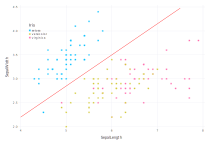
\includegraphics[width=\textwidth]{iris_plot.pdf}
        \end{center}
    \end{columns}
    \vfill
    \begin{itemize}
        \item A \emph{setosa} model: $ - 0.40 -0.65x_1 + 1.00x_2  > 0.00$.
        \item A general \textbf{model template}:
              $$
                  f_\theta(\vec{x}) = \theta_0 + \theta_1 x_1 + \theta_2 x_2 + \theta_3 x_3 + \theta_4 x_4> 0
              $$
    \end{itemize}
\end{frame}
%
%===============================================================
\begin{frame}
    %-------------------------------------------------------------
    %[fragile]
    %-------------------------------------------------------------
    \frametitle{Assumptions of Machine Learning}
    %-------------------------------------------------------------
    \begin{itemize}
        \item Each instance is described in a \textbf{single row} by a \textbf{fixed set of features}
              $$
                  \begin{array}{cccc|c}
                      \mathbf{x_1} & \mathbf{x_2} & \ldots & \mathbf{x_n} & \mathbf{y} \\
                      \hline
                      x_{11}       & x_{21}       & \ldots & x_{n1}       & y_1        \\
                                   &              & \vdots                             \\
                      x_{1m}       & x_{2m}       & \ldots & x_{nm}       & y_m        \\
                  \end{array}
                  .$$
        \item Instances are \textbf{independent} of one another, \textbf{given the model}
              $$
                  y = f_\theta(\vec{x}).
              $$
        \item Parameters \textbf{minimize estimation error} \emph{e.g.}
              $$
                  \hat{\theta} = \arg\min_\theta \sum_i \norm{y_i - f_\theta(\vec{x_{i}})}.
              $$
    \end{itemize}
\end{frame}
%
%===============================================================
\begin{frame}
    %-------------------------------------------------------------
    %[fragile]
    %-------------------------------------------------------------
    \frametitle{Failing Assumptions\hfill~1/2}
    %-------------------------------------------------------------
    \vfill
    \begin{columns}[c]
        \column{0.5\textwidth}
        $$
            \begin{array}{ccc}
                \text{student} & \text{course} & \text{grade} \\
                \hline
                s_1            & c_1           & a            \\
                s_2            & c_1           & c            \\
                s_1            & c_2           & b            \\
                s_2            & c_3           & b            \\
                s_3            & c_2           & b            \\
                s_4            & c_3           & b            \\
                s_3            & c_4           & X            \\
                s_4            & c_4           & Y            \\
            \end{array}
        $$
        \column{0.5\textwidth}
        \emph{Infer $X \succ_g Y$.}

        \bigskip
        ``\emph{Proof.}'' 

            \bigskip
            $s_1 \succ_s s_2$ (rows 1 \& 2)\\ so $c_2 \succ_c c_3$ (3 \& 4). 
            
            \bigskip
            Then $s_3 \succ_s s_4$ (5 \& 6)\\ therefore $X \succ_g Y\qed$.
    \end{columns}
    \vfill
    \begin{itemize}
        \item Instances are not independent.
        \item Small dataset, so \emph{no statistics}.
    \end{itemize}
\end{frame}
%
%===============================================================
\begin{frame}
    %-------------------------------------------------------------
    %[fragile]
    %-------------------------------------------------------------
    \frametitle{Failing Assumptions\hfill~2/2}
    %-------------------------------------------------------------
    \footnotesize
    \begin{center}
        \textbf{Prompt:} Given \texttt{f(machine) = e}, \texttt{f(learning) = g} and \texttt{f(algorithm) = m}, what is the value of \texttt{f(ksadbf)}?
    \end{center}

    \vfill
    \begin{columns}[t]
        \scriptsize
        \column{0.35\textwidth}
        $$
            \begin{array}{r|l}
                \textbf{input} & \textbf{output} \\
                \hline
                machine        & e               \\
                learning       & g               \\
                algorithm      & m               \\
                ksadbf         & ?
            \end{array}
        $$

        \bigskip
        \textbf{Bard:} \tt f(ksadbf) = 11.

        We can see that the value of f(x) is simply the first letter of x minus 96.

        \column{0.65\textwidth}

        \textbf{ChatGPT:} \tt The information provided seems to define a function $f$ where certain inputs are associated with specific outputs. Based on the given information:
        \begin{itemize}
            \item $f(\text{machine}) = e$
            \item $f(\text{learning}) = g$
            \item $f(\text{algorithm}) = m$
        \end{itemize}
        However, there is no information given about \( f(\text{ksadbf}) \). Without additional information or a specific rule that determines the output for \( f(\text{ksadbf}) \), \emph{it is not possible to determine its value}.
        %
        If there is a pattern or rule for how the outputs are assigned based on the inputs, you would need to provide that information for me to help determine the value of \( f(\text{ksadbf}) \).
    \end{columns}

    \vfill
    \begin{center}
        No help from state-of-the-art Natural Language Processing or LLMs.
    \end{center}
\end{frame}
%
%===============================================================
\begin{frame}
    %-------------------------------------------------------------
    %[fragile]
    %-------------------------------------------------------------
    \frametitle{Where Machine Learning Fails}
    %-------------------------------------------------------------
    \begin{itemize}
        \item No \emph{interpretability}: large models ($\dim \theta \sim \text{millions}$) are \alert{not understandable by humans}.
        \item Need for \emph{large number of training} examples.
        \item Unfit for \emph{multiple relations}, \emph{intersample dependencies} and \emph{variable features}: The \textit{Students, Courses and Results} and \emph{Last Letter} examples.
        \item Poor \emph{generalization}: A model trained in the iris dataset is useless in any other domain.
        \item \alert{No use of background knowledge}.
    \end{itemize}
\end{frame}
%
%===============================================================
%
\section{Logic Programming}
%
%===============================================================
\begin{frame}
    %------------------------------------------------------------- %-------------------------------------------------------------
    \frametitle{}
    %-------------------------------------------------------------
    \begin{center}
        \vfill
        {\huge\bf Logic Programming}
    \end{center}
    \vfill
    \begin{itemize}
        \item An Example of Logic Programming.
        \item Inductive Logic Programming.
        \item Where ILP Fails.
    \end{itemize}
    \vfill
    %-------------------------------------------------------------
\end{frame}
%
%===============================================================
\begin{frame}
    %-------------------------------------------------------------
    [fragile]
    %-------------------------------------------------------------
    \frametitle{An Example of Logic Programming}
    %-------------------------------------------------------------
    \begin{columns}[c]
        \column{0.4\textwidth}
        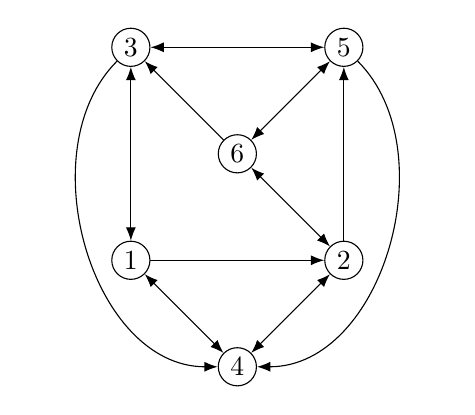
\begin{tikzpicture}[>=Latex]
            \node[vert] (v6) {6};
            \node[vert, above left = of v6] (v3) {3};
            \node[vert, above right = of v6] (v5) {5};
            \node[vert, below left = of v6] (v1) {1};
            \node[vert, below right = of v6] (v2) {2};
            \node[vert, below right = of v1] (v4) {4};
            \draw[->] (v6) to (v3);
            \draw[<->] (v6) to (v5);
            \draw[<->] (v6) to (v2);
            \draw[<->] (v3) to (v5);
            \draw[<->] (v3) to (v1);
            \draw[->] (v3) to[bend right, out=225, in =180,relative=false] (v4);
            \draw[->] (v1) to (v2);
            \draw[<->] (v1) to (v4);
            \draw[->] (v2) to (v5);
            \draw[<->] (v2) to (v4);
            \draw[->] (v5) to[bend left, out=-45, in=0,relative=false] (v4);
        \end{tikzpicture}
        \column{0.6\textwidth}
        \scriptsize
        \begin{lstlisting} 
node(1..6).

edge(1,2). edge(2,4). edge(3,1).
edge(4,1). edge(5,3). edge(6,2).
edge(1,3). edge(2,5). edge(3,4).
edge(4,2). edge(5,4). edge(6,3).
edge(1,4). edge(2,6). edge(3,5).
edge(5,6). edge(6,5).

col(r). col(b). col(g).

1 { color(X,C) : col(C) } 1 :- node(X).
:- edge(X,Y), color(X,C), color(Y,C).

#show color/2.
        \end{lstlisting}
    \end{columns}
    \vfill
    \scriptsize
    \begin{lstlisting}    
color(2,b) color(1,g) color(4,r) color(3,b) color(5,g) color(6,r)
color(1,r) color(2,b) color(4,g) color(3,b) color(5,r) color(6,g)
color(1,r) color(2,g) color(4,b) color(3,g) color(5,r) color(6,b)
color(1,b) color(2,g) color(4,r) color(3,g) color(5,b) color(6,r)
color(2,r) color(1,g) color(4,b) color(3,r) color(5,g) color(6,b)
color(2,r) color(1,b) color(4,g) color(3,r) color(5,b) color(6,g)
    \end{lstlisting}
\end{frame}
%
%===============================================================
\begin{frame}
    %-------------------------------------------------------------
    %[fragile]
    %-------------------------------------------------------------
    \frametitle{Inductive Logic Programming}
    %-------------------------------------------------------------
    \small

    \vfill
    \begin{center}
        Learning Logic Programs from Examples.
    \end{center}

    \vfill
    \alert{Generate rules} that\ldots
    \begin{itemize}
        \item use \textbf{background knowledge}
        $$
            \begin{aligned}
                 & parent(john,mary),  &  & parent(david,steve), \\
                 & parent(kathy,mary), &  & female(kathy),       \\
                 & male(john),         &  & male(david).
            \end{aligned}
        $$
        \item to entail all the \textbf{positive examples}, $father(john,mary), father(david,steve)$,
        \item but none of the \textbf{negative examples}. $father(kathy,mary), father(john,steve)$,
        
    \end{itemize}

    \vfill
    A \textbf{solution} is $$father(X,Y) \leftarrow parent(X,Y) \wedge male(X).$$

\end{frame}
%
%===============================================================
\begin{frame}
    %-------------------------------------------------------------
    %[fragile]
    %-------------------------------------------------------------
    \frametitle{Where Logic Programming Fails}
    %-------------------------------------------------------------
    \begin{center}
        Meanwhile, in the \textbf{real world}, samples are \emph{incomplete} and come with \emph{noise}.
    \end{center}
    \vfill
    \textbf{Logic inference is \alert{fragile}}: a mistake in the transcription of a fact is dramatic to the consequences:
    \begin{itemize}
        \item $parent(david,mary)$.
        \item $parent(jonh,mary)$.
    \end{itemize}
    \vfill
    \begin{center}
        The statistic essence of machine learning provides \alert{robustness}.
    \end{center}
\end{frame}
%
%===============================================================
%
\section{Probabilistic Logic Programming}
%
%===============================================================
%
\begin{frame}
    %------------------------------------------------------------- %-------------------------------------------------------------
    \frametitle{}
    %-------------------------------------------------------------
    \vfill
    \begin{center}
        {\huge\bf Probabilistic Logic Programming}
    \end{center}
    \vfill
    \begin{itemize}
        \item Define distributions from logic programs.
        \item Stochastic ASP: Specifying distributions.
    \end{itemize}
    \vfill
    %-------------------------------------------------------------
\end{frame}
%
%===============================================================
\begin{frame}
    %-------------------------------------------------------------
    %[fragile]
    %-------------------------------------------------------------
    \frametitle{Probabilistic Logic Programs (PLPs)}
    %-------------------------------------------------------------
    \small

    \vfill
    \begin{center}
        Logic programs \textbf{annotated} with probabilities.
    \end{center}

    \vfill
    \begin{columns}[c]

        \column{0.4\textwidth}
        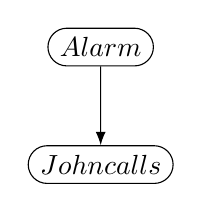
\begin{tikzpicture}[>=Latex]
            \node[draw, rounded rectangle] (A) {$Alarm$};
            \node[draw, rounded rectangle, below = of A] (J) {$Johncalls$};
            \draw[->] (A) to (J);
        \end{tikzpicture}

        \column{0.6\textwidth}
        $
            \begin{aligned}
                alarm:0.00251, &                       \\
                johncalls:0.9  & \leftarrow alarm,     \\
                johncalls:0.05 & \leftarrow \neg alarm
            \end{aligned}
        $
    \end{columns}

    \vfill
    \begin{itemize}
        \item \alert{$alarm:0.00251$} is $alarm \vee \neg alarm$ plus $P(Alarm = true) = 0.00251$.
        \item \alert{$johncalls:0.9 \leftarrow alarm$} is
              $$P\del{Johncalls = true \middle| Alarm = true} = 0.9$$
    \end{itemize}

    \vfill
    \begin{center}
        Any bayesian network can be represented by a PLP.
    \end{center}
\end{frame}
%
%===============================================================
\begin{frame}
    %-------------------------------------------------------------
    %[fragile]
    %-------------------------------------------------------------
    \frametitle{Distributions from Logic Programs}
    %-------------------------------------------------------------
    \vfill
    The program
    $$
        \begin{aligned}
            alarm:0.00251, &                       \\
            johncalls:0.9  & \leftarrow alarm,     \\
            johncalls:0.05 & \leftarrow \neg alarm
        \end{aligned}
    $$
    entails four possible models (or worlds):
    $$
        \begin{array}{r|r}
            \text{model}               & \text{probability} \\
            \hline
            alarm, johncalls           & 0.002259   \\
            alarm, \neg johncalls      & 0.000251   \\
            \neg alarm, johncalls      & 0.049874   \\
            \neg alarm, \neg johncalls & 0.947616   \\
        \end{array}
    $$
    \begin{itemize}
        \item \alert{\textbf{Models}} are special sets of \emph{literals} \textbf{entailed} from the program.
        \item Probabilities \emph{propagate} from facts, through rules.
    \end{itemize}
    \vfill
\end{frame}
%
%===============================================================
\begin{frame}
    %-------------------------------------------------------------
    %[fragile]
    %-------------------------------------------------------------
    \frametitle{There's a Problem\ldots}
    %-------------------------------------------------------------
    \vfill
    The program
    $$
        \begin{aligned}
            alarm:0.00251,           &                  \\
            johncalls \vee marycalls & \leftarrow alarm
        \end{aligned}
    $$
    entails three \alert{stable}  (\emph{i.e.}\ minimal) models
    $$
        \begin{array}{r|l}
            \text{model}     & \text{probability} \\
            \hline
            alarm, johncalls & x                  \\
            alarm, marycalls & y                  \\
            \neg alarm       & 0.99749
        \end{array}
    $$
    but \textbf{no single way to set $x,y$}.
    \vfill
    \begin{center}
        Some \emph{Probabilistic Logic Programs} define more than one joint distribution.
    \end{center}
\end{frame}
%
%===============================================================
\begin{frame}
    %-------------------------------------------------------------
    %[fragile]
    %-------------------------------------------------------------
    \frametitle{\ldots and an Oportunity}
    %-------------------------------------------------------------
    \begin{center}
        Some \emph{PLP}s define more than one joint distribution.
    \end{center}
    \vfill
    \begin{itemize}
        \item There is \textbf{no single probability assignment} from the facts stable models: $x,y \in \intcc{0,1}$.
        \item But any assignment is bound by Kolmogorov's axioms, and \textbf{forms equations} such as:
              $$x + y = P\del{alarm}.$$
        \item Existing \textbf{data can be used to estimate the unknowns} in those equations.
    \end{itemize}
    \vfill
\end{frame}
%
%===============================================================
\begin{frame}
    %-------------------------------------------------------------
    %[fragile]
    %-------------------------------------------------------------
    \frametitle{Stable Models, Events and Probabilities}
    %-------------------------------------------------------------
    \vfill
    \begin{center}
        What are we talking about?
    \end{center}
    \vfill
    \begin{itemize}
        \item A logic program has \textbf{atoms} (and \textbf{literals}) and \textbf{rules}:
            $$
            \begin{aligned}
                &male(john), \neg parent(kathy,mary), \\
                &father(X, Y) \leftarrow parent(X, Y) \wedge male(X).
            \end{aligned}
            $$
        \item A \alert{\textbf{stable model}} is a \textbf{minimal} model that contains:
              \begin{itemize}
                  \item program's \emph{facts}: $parent(john,mary),~male(john)$.
                  \item consequences, by the \emph{rules}: $father(john,mary)$.
              \end{itemize}
        \item Some programs have more than one model:
              \begin{tabular}{c|c}
                  \textbf{Logic Program} & \textbf{Stable Models} \\
                  \hline
                  $a \vee \neg a,  b \vee c \leftarrow a$
                                         &
                  $\set{\neg a}, \set{a, b}, \set{a, c}$
              \end{tabular}
    \end{itemize}
    \vfill
    \begin{center}
        How to propagate probability from annotated facts to other \emph{events}?
    \end{center}
\end{frame}
%
%===============================================================
\begin{frame}
    %-------------------------------------------------------------
    %[fragile]
    %-------------------------------------------------------------
    \frametitle{Logic Programs and Probabilities}
    %-------------------------------------------------------------
    % \vfill
    % \begin{center}
    %     The \textbf{space of events}, $\Omega$, is the set of all sets of literals. 
    % \end{center}
    \vfill
    \begin{itemize}
        \item Consider the literals of a logic program $$L = \set{a_1, \ldots a_n, \neg a_1, \ldots \neg a_n}.$$
        \item Any model of that program is a (consistent) subset of $L$.
        \item Let $\Omega = \mathbf{P}\del{L}$, \emph{i.e.} an \alert{event} $e$ is a subset of $L$, $e \subseteq L$.
              \begin{itemize}
                  \item Setting a probability for some events seems straightforward: $P\del{\neg alarm} = 0.997483558$.
                  \item For others, not so much:
                        \begin{itemize}
                            \item $P\del{alarm, johncalls}$, $P\del{johncalls, marycalls, alarm}$, $P\del{marycalls}$?
                            \item $P\del{alarm, \neg alarm}$, $P\del{\neg marycalls}$?
                        \end{itemize}
              \end{itemize}
    \end{itemize}
    \vfill
    \begin{center}
        How to \alert{propagate} probability from \emph{facts} to \emph{consequences} or other \emph{events}?
    \end{center}
\end{frame}
%
\newcommand{\diagram}{
    \resizebox{!}{24ex}{
        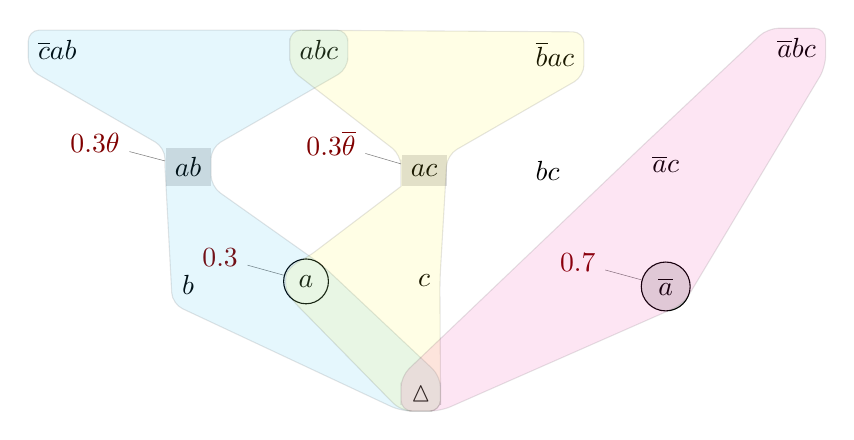
\begin{tikzpicture}%[scale=0.6, every node/.style={scale=0.6}]
            \node[event] (E) {$\emptyevent$};
            \node[tchoice, above left = of E, pin={[red!50!black]175:$0.3$}] (a) {$a$};
            \node[smodel, above left = of a, pin={[red!50!black]175:$0.3\theta$}] (ab) {$ab$};
            \node[smodel, above right = of a, pin={[red!50!black]175:$0.3\co{\theta}$}] (ac) {$ac$};
            \node[event, below = of ab] (b) {$b$};
            \node[event, below = of ac] (c) {$c$};
            \node[event, above right = of ab] (abc) {$abc$};
            \node[event, above left = of ab] (abC) {$\co{c}ab$};
            \node[event, above right = of ac] (aBc) {$\co{b}ac$};
            \node[indep, right = of ac] (bc) {$bc$};
            \node[tchoice, smodel, below right = of bc, pin={[red!50!black]175:$0.7$}] (A) {$\co{a}$};
            \node[event, above = of A] (Ac) {$\co{a}c$};
            \node[event, above right = of Ac] (Abc) {$\co{a}bc$};
            % ----
            \path[draw, rounded corners, fill=cyan, opacity=0.1]
            (ab.west) --
            (ab.north west) --
            %
            (abC.south west) --
            (abC.north west) --
            (abC.north) --
            %
            (abc.north east) --
            (abc.east) --
            (abc.south east) --
            %
            (ab.north east) --
            (ab.east) --
            (ab.south east) --
            %
            (a.north east) --
            %
            (E.north east) --
            (E.east) --
            (E.south east) --
            (E.south) --
            (E.south west) --
            %
            (b.south west) --
            %
            (ab.west)
            ;
            % ----
            \path[draw, rounded corners, fill=yellow, opacity=0.1]
            (ac.south west) --
            (ac.west) --
            (ac.north west) --
            %
            (abc.south west) --
            (abc.west) --
            (abc.north west) --
            %
            (aBc.north east) --
            (aBc.east) --
            (aBc.south east) --
            %
            (ac.north east) --
            %
            (c.east) --
            %
            (E.east) --
            (E.south east) --
            (E.south) --
            (E.south west) --
            %
            (a.south west) --
            (a.west) --
            (a.north west) --
            (a.north) --
            %
            (ac.south west)
            ;
            % ----
            \path[draw, rounded corners, fill=magenta, opacity=0.1]
            % (A.north west) --
            %
            (Ac.north west) --
            %
            (Abc.north west) --
            (Abc.north) --
            (Abc.north east) --
            (Abc.south east) --
            %
            % (Ac.north east) --
            % (Ac.east) --
            %
            % (A.east) --
            (A.south east) --
            %
            (E.south east) --
            (E.south) --
            (E.south west) --
            (E.west) --
            (E.north west) --
            %
            (Ac.north west)
            ;
        \end{tikzpicture}
    }
}
%
%===============================================================
\begin{frame}
    %-------------------------------------------------------------
    %[fragile]
    %-------------------------------------------------------------
    \frametitle{Classes of Events}
    %-------------------------------------------------------------
    \small

    \vfill
    \begin{center}
        \diagram
    \end{center}

    \vfill
    \begin{center}
        \begin{tabular}{lr}
            $\begin{aligned}
                     \probfact{0.3}{a}       \\
                     b \vee c & \leftarrow a
                 \end{aligned}$
             &
            $\co{a} = \set{\neg a}, ab = \set{a, b}, ac = \set{a, c}$
        \end{tabular}
    \end{center}

    \vfill
    \begin{itemize}
        \item Define \alert{equivalence classes} for all events, based on $\subseteq, \supseteq$ relations with the \textbf{stable models}.
        \item This example shows $6$ out of $2^3 + 1$ classes.
    \end{itemize}
\end{frame}
%
%===============================================================
\begin{frame}
    %-------------------------------------------------------------
    %[fragile]
    %-------------------------------------------------------------
    \frametitle{Probabilities for all Events}
    %-------------------------------------------------------------
    \vfill
    \begin{center}
        \diagram
    \end{center}
    \vfill
    \footnotesize
    \begin{enumerate}
        \item Set \alert{weights} in the stable models (shaded nodes), using parameters when needed: $\mu\del{\co{a}} = 0.7; \mu\del{ab} = 0.3\theta; \mu\del{ac}=0.3\del{1 - \theta}$
        \item Assume that the stable models are \alert{disjoint events}.
        \item Define \alert{weight of an event} as the sum of the weights of the related stable models.
        \item Normalize weights to get a (probability) \alert{distribution}.
    \end{enumerate}
\end{frame}
%
%===============================================================
\begin{frame}
    %-------------------------------------------------------------
    %[fragile]
    %-------------------------------------------------------------
    \frametitle{Probabilities for all Events}
    %-------------------------------------------------------------
    \vfill
    % \begin{center}
    %     \diagram
    % \end{center}
    % \vfill
    % \scriptsize

    \begin{equation*}
        \begin{array}{clr|cc|cc}
            & \stablecore{e}
            & \# \class{e}
            & \pw{\class{e}}
            & \pw{e}
            & \pr{E = e}
            & \pr{E \in \class{e}}
            \\
            \hline
            %
            & \inconsistent
            & 37
            & 0
            & 0
            & 0
            & 0
            \\[4pt]
            %
            \square 
            & \indepclass
            & 9
            & 0
            & 0
            & 0
            & 0
            \\[4pt]
            %
            {\color{magenta!20}\blacksquare }
            & \co{a}
            & 9
            & \frac{7}{10}
            & \frac{7}{90}
            & \frac{7}{207}
            & \frac{7}{23}
            \\[4pt]
            %
            {\color{cyan!20}\blacksquare }
            & ab
            & 3
            & \frac{3}{10}\theta
            & \frac{1}{10}\theta
            & \frac{1}{23}\alert{\theta}
            & \frac{3}{23}\theta
            \\[4pt]
            %
            {\color{yellow!20}\blacksquare }
            & ac
            & 3
            & \frac{3}{10}\co{\theta}
            & \frac{1}{10}\co{\theta}
            & \frac{1}{23}\alert{\co{\theta}}
            & \frac{3}{23}\co{\theta}
            \\[4pt]
            %
            & \co{a}, ab
            & 0
            & \frac{7 + 3\theta}{10}
            & 0
            & 0
            & 0
            \\[4pt]
            %
            & \co{a}, ac
            & 0
            & \frac{7 + 3\co{\theta}}{10}
            & 0
            & 0
            & 0
            %
            \\[4pt]
            %
            {\color{green!20}\blacksquare }
            & ab, ac
            & 2
            & \frac{3}{10}
            & \frac{3}{20}
            & \frac{3}{46}
            & \frac{3}{23}
            \\[4pt]
            %
            {\color{gray!20}\blacksquare }
            & \co{a}, ab, ac
            & 1
            & 1
            & 1
            & \frac{10}{23}
            & \frac{10}{23}
            \\[4pt]
            %
            \hline
            &
            & 64
            & 
            & Z = \frac{23}{10}
            &
            %& \Sigma = 1
        \end{array}
    \end{equation*}
\end{frame}
%
%===============================================================
\begin{frame}
    %-------------------------------------------------------------
    %[fragile]
    %-------------------------------------------------------------
    \frametitle{Estimating the Parameters}
    %-------------------------------------------------------------
    A \alert{sample} can be used to estimate the parameters $\theta$, by minimizing
    \begin{equation*}
        \err{\theta} := \sum_{e\in\fml{E}} \del{\pr{E = e\given \Theta = \theta} - \pr{S = e}}^2.\label{eq:err.e.s}
    \end{equation*}
    where
    \begin{itemize}
        \item $\fml{E}$ is the set of all events,
        \item $\pr{E\given \Theta}$ the \textbf{model+parameters} based distribution, 
        \item $\pr{S}$ is the \textbf{empiric} distribution from the given sample.
    \end{itemize}  
\end{frame}
%
%===============================================================
\begin{frame}
    %-------------------------------------------------------------
    %[fragile]
    %-------------------------------------------------------------
    \frametitle{Behind Parameter Estimation}
    %-------------------------------------------------------------
    \vfill
    So, we can derive a distribution $\pr{E\given \Theta = \hat{\theta}}$ from a program $P$ and a sample $S$.
    \begin{itemize}
        \item The sample defines an empiric distribution $\pr{S}$\ldots
        \item \ldots that is used to estimate $\theta$ in $\pr{E\given \Theta}$\ldots
        \item \ldots and \alert{score the program} $P$ w.r.t.\ that sample using, \emph{e.g.} the $\err{}$ function.
    \end{itemize}
    \vfill

\end{frame}
%
%===============================================================
\begin{frame}
    %-------------------------------------------------------------
    %[fragile]
    %-------------------------------------------------------------
    \frametitle{Back to Inductive Logic Programming}
    %-------------------------------------------------------------
    \vfill
    Recall the \emph{Learning Logic Programs from Examples} setting:
    \begin{itemize}
        \item Given \textbf{positive} and \textbf{negative} examples, and \textbf{background knowledge}\ldots
        \item find a \textbf{program}\ldots
              \begin{itemize}
                  \item \ldots using the facts and relations from the \textbf{BK}\ldots
                  \item \ldots such that \textbf{all the PE} and \textbf{none the NE} examples are entailed.
              \end{itemize}
    \end{itemize}
    \vfill
    \begin{quotation}
        Given a sample of events, and a set of programs, \alert{the score} of those programs (w.r.t. the sample) \alert{can be used in evolutionary algorithms} while searching for better solutions.
    \end{quotation}
\end{frame}
%
%===============================================================
%
\section{In Conclusion}
%
%===============================================================
%
\begin{frame}
    %------------------------------------------------------------- %-------------------------------------------------------------
    \frametitle{}
    %-------------------------------------------------------------
    \vfill
    \begin{center}
        {\huge\bf In Conclusion}
    \end{center}
    \vfill
    %-------------------------------------------------------------
\end{frame}
%
%===============================================================
\begin{frame}
    %-------------------------------------------------------------
    %[fragile]
    %-------------------------------------------------------------
    % \frametitle{In Conclusion}
    %-------------------------------------------------------------
    \begin{itemize}
        \item \textbf{Machine Learning} has limitations.
        \item As does \textbf{Inductive Logic Programming}.
        \item But, distributions can be defined by \textbf{Stochastic Logic Programs}.
    \end{itemize}
\end{frame}
%
%===============================================================
\begin{frame}
    %-------------------------------------------------------------
    %[fragile]
    %-------------------------------------------------------------
    % \frametitle{In Conclusion}
    %-------------------------------------------------------------
    Distributions can be defined by \textbf{Stochastic Logic Programs}. Here we:
    \begin{enumerate}
        \item Look at the program's \textbf{stable models} and
        \item Use them to partition the \textbf{events} and then
        \item Using annotated probabilities, define:
        \begin{enumerate}
            \item a finite \textbf{measure}\ldots
            \item that, normalized, is a  \textbf{distribution} on all events.
        \end{enumerate}
    \end{enumerate}
\end{frame}
%
%===============================================================
\begin{frame}
    %-------------------------------------------------------------
    %[fragile]
    %-------------------------------------------------------------
    % \frametitle{In Conclusion}
    %-------------------------------------------------------------
    Distributions can be defined by \textbf{Stochastic Logic Programs}.
    \begin{itemize}
        \item These distributions might have some \textbf{parameters}, due to indeterminism in the program.
        \item A \textbf{sample} can be used to estimate those parameters\ldots
        \item \ldots and \textbf{score} programs concurring to describe it.
        \item This score a key ingredient in \textbf{evolutionary algorithms}.
    \end{itemize}
    \begin{quotation}
        \ldots and a step towards the \alert{induction of stochastic logic programs} using \textbf{data} and \textbf{background knowledge}.
    \end{quotation}
\end{frame}
%
%===============================================================
\begin{frame}
    %-------------------------------------------------------------
    %[fragile]
    %-------------------------------------------------------------
    \frametitle{Future Work}
    %-------------------------------------------------------------
    \vfill
    \begin{center}
        Induction of Stochastic Logic (ASP) Programs.
    \end{center}
    \vfill
    \begin{enumerate}
        \item \textbf{Meta-programming:} formal rules for rule generation.
        \item \textbf{Generation}, \textbf{Combination} and \textbf{Mutation} operators.
        \item \textbf{Complexity.}
        \item \textbf{Applications.}
        \item \textbf{Profit.}
    \end{enumerate}
    \vfill
\end{frame}
%
%===============================================================
\begin{frame}
    %-------------------------------------------------------------
    %[fragile]
    %-------------------------------------------------------------
    \frametitle{}
    %-------------------------------------------------------------
    \begin{center}
        \vfill
        {\huge\alert{\bf Thank You!}}
        \vfill
        Questions?
    \end{center}
\end{frame}
%
%===============================================================
\begin{frame}
    %-------------------------------------------------------------
    %[fragile]
    %-------------------------------------------------------------
    \frametitle{References}
    \begin{itemize}
        \item \href{https://arxiv.org/abs/1801.00631}{Gary Marcus, \emph{Deep Learning: A Critical Appraisal}, 2018}.
        \item \href{https://arxiv.org/abs/1911.01547}{François Chollet, \emph{On the Measure of Intelligence}, 2019}.
        \item \href{https://arxiv.org/abs/1801.00631}{Bengio \emph{et al.}, \emph{A Meta-Transfer Objective for Learning to Disentangle Causal Mechanisms}, 2019}.
        \item \href{https://arxiv.org/abs/1801.00631}{Cropper \emph{et al.}, \emph{Turning 30: New Ideas in Inductive Logic Programming}, 2020}.
        \item \href{https://doi.org/10.1201/9781003427421}{Fabrizio Riguzzi, \emph{Foundations of Probabilistic Logic Programming }, 2023}.
    \end{itemize}
    %-------------------------------------------------------------
\end{frame}
%
\end{document}
%
%===============================================================
\begin{frame}
    %-------------------------------------------------------------
    %[fragile]
    %-------------------------------------------------------------
    \frametitle{TITLE}
    %-------------------------------------------------------------
\end{frame}
%


